\documentclass[11pt,letterpaper]{article}
\usepackage[margin=1in]{geometry}
\usepackage{graphicx}
\usepackage{hyperref}
\usepackage{booktabs}
\usepackage{xcolor}
\usepackage{listings}
\usepackage{longtable}

\graphicspath{{figures/}}

\lstset{
  basicstyle=\ttfamily\small,
  frame=single,
  breaklines=true,
  columns=fullflexible,
  backgroundcolor=\color{gray!8}
}

\hypersetup{colorlinks=true, urlcolor=blue, linkcolor=blue, citecolor=blue}

\title{MusX User and Developer Manual\\[2pt]\large A browser-based node patcher for sound and music}
\author{Paul Fishwick and Claude Code}
\date{July 2026}

\begin{document}

\maketitle
\tableofcontents
\newpage

\section{Introduction}

MusX is a single-page, browser-based \emph{node patcher} for building sounds and music.
A patch is a graph of typed objects (``nodes'') wired together by cables; the graph is
evaluated by the Web Audio API~\cite{webaudio} through the Tone.js library~\cite{tonejs}.
MusX evolved from studying two seminal visual dataflow environments for computer music:
Miller Puckette's Pure Data (Pd)~\cite{puckette} and Cycling~'74's Max/MSP~\cite{maxmsp}.
From those systems MusX borrows the central idea that a musician builds an instrument by
\emph{wiring objects together} rather than writing a program in text, along with specific
conventions such as the tilde (\texttt{\~{}}) suffix on signal-rate objects, inlets on the
top of a box and outlets on the bottom, and the distinction between audio signals and
control messages. MusX deliberately keeps a much smaller object set than Pd or Max, aiming
for a simple but comprehensive core that runs with no installation in any modern browser.
More recently MusX has grown a \emph{sound-transformation} side inspired by the Composers
Desktop Project (CDP)~\cite{cdp} and its node-based front end SoundThread~\cite{soundthread}.
Where CDP transforms recorded sound offline through command-line tools, MusX reimplements
the same ideas as \emph{real-time} Web Audio objects: soundfile and microphone inputs
(Section~\ref{sec:sources}) feeding granular and other transformations that process live.

As shown in Figure~\ref{fig:interface}, the workspace is a dot-grid canvas populated with
object boxes. Audio cables are drawn thick and orange; control cables are thin and green.
A toolbar across the top hosts the global controls (audio on/off, transport, tempo, master
level, and patch file management).

\begin{figure}[h]
\centering
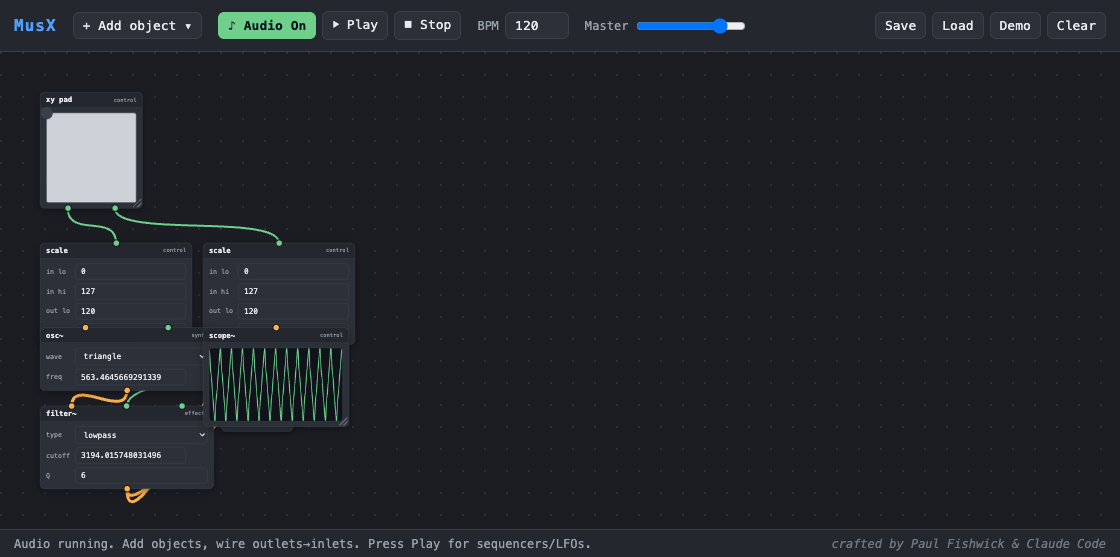
\includegraphics[width=0.95\textwidth]{interface.png}
\caption{The MusX workspace with the ``XY Synth'' patch loaded --- an \texttt{xy pad}
drives a \texttt{tri\~{}} oscillator through two \texttt{scale} objects and a resonant
\texttt{filter\~{}} into the output, with a \texttt{scope\~{}} showing the waveform. This
patch reproduces the subtractive-synth example from the Max/MSP product page~\cite{maxmsp}.}
\label{fig:interface}
\end{figure}

\subsection{Design Goals}

\begin{itemize}
  \item \textbf{No build step, no install.} MusX is plain HTML, CSS, and ES-module
        JavaScript. Tone.js is vendored locally; nothing is fetched at runtime except the
        optional Python runtime (Section~\ref{sec:code}).
  \item \textbf{Local-first.} Everything runs in the browser on the user's machine.
  \item \textbf{Signal vs.\ message.} As in Pd and Max, MusX separates audio signals
        (continuous, sample-rate) from control messages (discrete events).
  \item \textbf{One object = one definition.} Adding a new object is a single registry
        entry; the graph engine never special-cases an object type
        (Section~\ref{sec:dev}).
  \item \textbf{Resizable, legible UI.} Every graphical object can be resized, and any
        object carrying a frequency shows the corresponding musical note.
\end{itemize}

\section{Installation and Setup}

MusX has been developed and tested on macOS with a Chromium-based browser. Because it uses
ES modules, it must be served over HTTP rather than opened from the filesystem. The
repository root contains two shell scripts:

\begin{lstlisting}
./start   # serves http://localhost:8123 (prints the URL)
./stop    # stops the server (robust: stops by port even if the pid file is stale)
\end{lstlisting}

\texttt{./start} first frees its port: if any process (a stale server or another
application) is already listening there, it is closed before MusX takes the port. After
\texttt{./start}, open the printed \url{http://localhost:8123/index.html}. Click
\textbf{Start Audio} once (browsers require a user gesture before audio may begin), then
build a patch or load a demo.

\section{Interface Tour}
\label{sec:interface}

\subsection{Canvas and Objects}
Object boxes are dragged by their title bar. Each box has \emph{inlets} along the top and
\emph{outlets} along the bottom, drawn as small circles colour-coded by type: orange for
audio, green for control. Selecting a box (single click) and pressing \texttt{Delete}
removes it.

\subsection{Launch Default and Info Boxes}
On launch MusX loads the \textbf{Cathedral Pad} patch (Section~\ref{sec:richsound}) as a
ready-to-play default; a dismissable hint in the bottom-right corner notes that it can be
reloaded from \textbf{Demo $\rightarrow$ 11 Cathedral Pad}. A second box may appear in the
top-right corner: patches that carry an optional \texttt{credits} field (\texttt{text} +
\texttt{url}) --- such as the MIDI demos --- show that credit and a source link there.

\subsection{Auto-arrange}
\label{sec:autolayout}
The \textbf{Arrange} toolbar button (\texttt{Cmd/Ctrl+L}) tidies the current patch with an automatic
\emph{layered graph layout} --- the classic \textbf{Sugiyama} framework~\cite{sugiyama}, whose
practical form underlies tools such as Graphviz's \texttt{dot}~\cite{gansner}. It runs four phases:
(1) reverse a minimal set of back-edges so feedback loops form a directed acyclic graph;
(2) assign layers by longest path, so objects with no inputs sit on top and \texttt{dac\~{}} falls to
the bottom; (3) order objects within each row to reduce cable crossings (a median heuristic with
dummy nodes for long edges); and (4) assign coordinates, using isotonic regression to centre each
row under its neighbours without overlap. Because MusX puts inlets on top and outlets on the
bottom, the result reads as top-to-bottom signal flow. The built-in demos ship pre-arranged this
way; your own hand-placed layouts are only changed when you press the button.

\subsection{Adding Objects}
Objects are added from a two-level menu organised by function, shown in
Figure~\ref{fig:context-menu}. The menu opens either from the \textbf{+ Add object} button
in the toolbar or by right-clicking empty canvas; hovering a category reveals its objects
in a submenu. Right-click drops the new object where you clicked; the button drops it at a
staggered default position.

\begin{figure}[h]
\centering
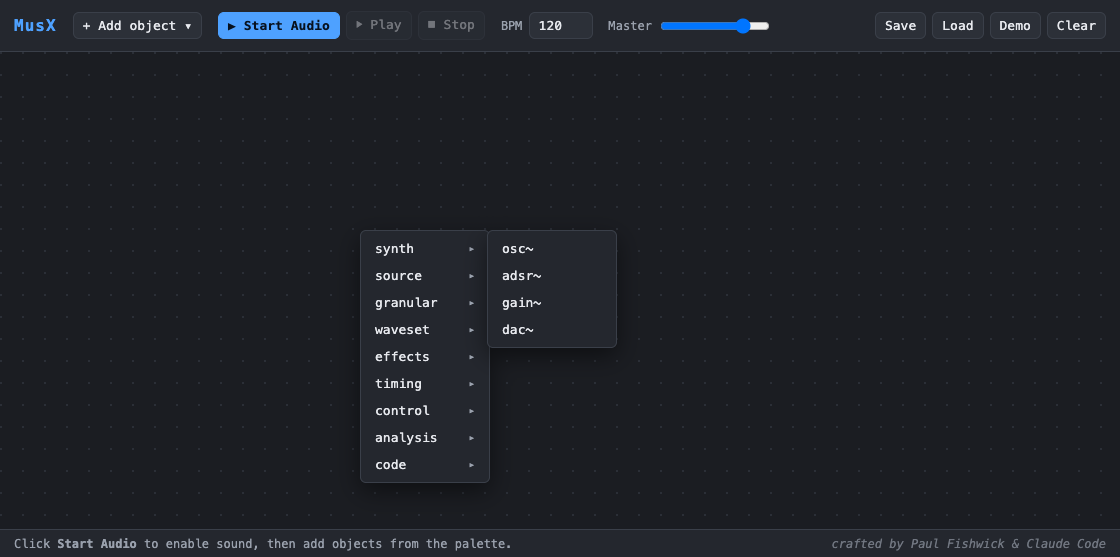
\includegraphics[width=0.7\textwidth]{context-menu.png}
\caption{The two-level ``Add object'' menu. Top level lists the functional
categories; hovering a category (here \texttt{synth}) reveals its objects to the right.}
\label{fig:context-menu}
\end{figure}

\subsection{Navigating: Pan, Zoom, and Fit}
\label{sec:navigate}
Patches can grow larger than the visible canvas. Scroll the mouse wheel to \textbf{zoom}
in and out (the zoom centres on the cursor); drag an empty part of the canvas (or use the
middle mouse button) to \textbf{pan}. Double-clicking empty canvas \textbf{fits} all
objects into view. Loading a patch automatically fits it, so an incoming patch is always
framed completely regardless of its size. Object dragging and object placement remain
accurate at any zoom level.

\subsection{Wiring and Deleting Cables}
Drag from an outlet to an inlet to create a cable. Audio outlets connect only to audio
inlets and control to control; mismatches are rejected. A cable highlights red on hover;
clicking it deletes it.

\subsection{Resizing Graphical Objects}
Every graphical object --- \texttt{xy pad}, \texttt{scope\~{}}, \texttt{plot},
\texttt{keyboard}, \texttt{step seq}, \texttt{slider}, \texttt{bang}, \texttt{message}, and
\texttt{code} --- has a resize grip in its bottom-right corner. Dragging it rescales the
object (the keyboard rescales its keys, the grid its cells, canvases their drawing area).
The size is stored in the patch and restored on load.

\subsection{Frequency and Note Display}
Any object whose parameters include a frequency shows the nearest musical note and octave
immediately after the number, as in Figure~\ref{fig:note-labels}. The note is shown only
when the frequency lies within a few cents of an equal-tempered pitch (for example
$440\,$Hz $\rightarrow$ A4, $1760\,$Hz $\rightarrow$ A6); frequencies that are not notes
leave the label blank. The on-screen keyboard labels each C with its octave (C3, C4,
\ldots).

\begin{figure}[h]
\centering
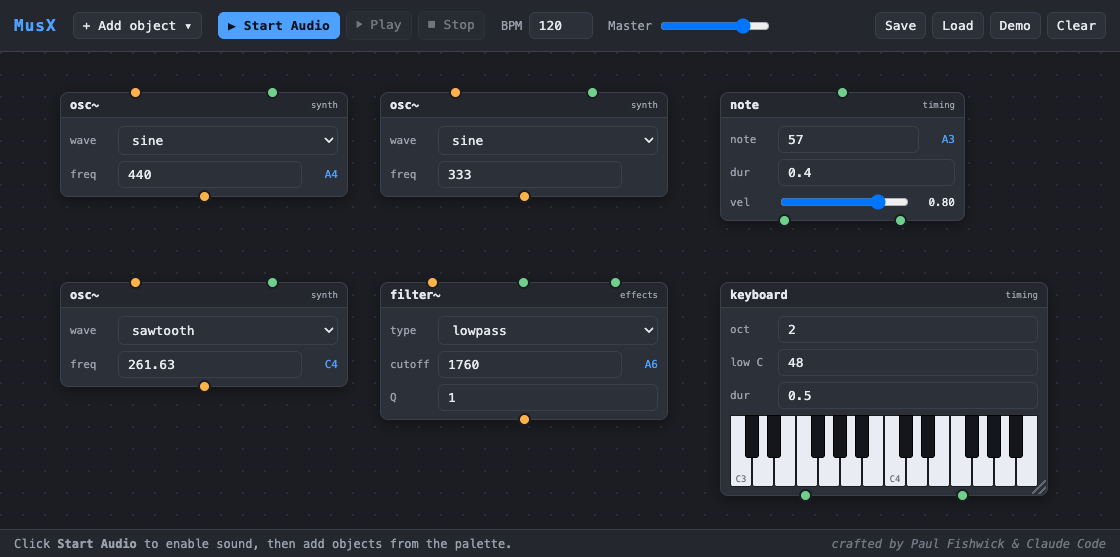
\includegraphics[width=0.95\textwidth]{note-labels.png}
\caption{Frequency-to-note display. The \texttt{osc\~{}} at $440\,$Hz shows A4 and at
$261.63\,$Hz shows C4; $333\,$Hz shows no note; the \texttt{filter\~{}} cutoff of
$1760\,$Hz shows A6; the \texttt{note} object shows A3. The keyboard's C keys are labelled
with their octaves.}
\label{fig:note-labels}
\end{figure}

\subsection{Audio Lifecycle: Start Audio, Play, Stop}
\textbf{Start Audio} unlocks the browser audio context and builds the live signal graph;
continuously sounding objects (free-running oscillators) begin immediately. \textbf{Play}
runs the global transport so that time-based objects (\texttt{metro}, \texttt{step seq},
the \texttt{funcgen} control sweep) fire, and ramps the master gain up. \textbf{Stop}
pauses the transport and ramps the master gain to zero. While stopped, \texttt{scope\~{}}
and \texttt{plot} draw a flat line so the visuals match the silence.

\subsection{Saving and Loading}
\textbf{Save} downloads the current patch as JSON (object types, positions, parameter
values, widget sizes, and all cables); \textbf{Load} restores one. Seven example patches
ship in \texttt{patches/} and are also available from the \textbf{Demo} button.

\section{Object Catalog}

Objects are grouped by function. Audio inlets/outlets are marked with a tilde in
the interface. Table~\ref{tab:objects} summarises the current set.

{\small
\begin{longtable}{@{}llp{7.4cm}@{}}
\caption{The MusX object catalog.}\label{tab:objects}\\
\toprule
\textbf{Category} & \textbf{Object} & \textbf{Function} \\
\midrule
\endfirsthead
\toprule
\textbf{Category} & \textbf{Object} & \textbf{Function} \\
\midrule
\endhead
source   & \texttt{sndfile\~{}} & Soundfile player: load/drag a WAV or pick a bundled sound; loop, varispeed, \texttt{trig}, and a Start-Mod random start offset (Section~\ref{sec:richsound}) \\
         & \texttt{sampler\~{}} & Play a sample chromatically (varispeed): \texttt{freq}$\rightarrow$playback rate about a \texttt{root} pitch, with a hold-to-sustain gate (Section~\ref{sec:richsound}) \\
         & \texttt{mic\~{}}     & Live microphone input; gain makeup and a live input-level (dB) meter \\
\midrule
synth    & \texttt{osc\~{}}   & Oscillator (sine/square/saw/triangle); freq control + audio-rate FM inlet \\
         & \texttt{unison\~{}} & Fat unison oscillator: up to 8 detuned, stereo-spread voices in one box (Section~\ref{sec:richsound}) \\
         & \texttt{pan\~{}}   & Equal-power stereo panner (position $-1\ldots1$) \\
         & \texttt{spat\~{}}  & 3D binaural panner (HRTF): $x$/$y$/$z$ place a source around the listener \\
         & \texttt{adsr\~{}}  & Attack--decay--sustain--release envelope (gated note-on/off); optional velocity$\rightarrow$amp \\
         & \texttt{gain\~{}}  & Amplitude / level \\
         & \texttt{dac\~{}}   & Audio output (to speakers via the master) \\
\midrule
effects  & \texttt{filter\~{}} & Lowpass/highpass/bandpass/notch with cutoff + Q \\
         & \texttt{delay\~{}}  & Feedback delay (time, feedback, wet) \\
         & \texttt{reverb\~{}} & Reverb (decay, pre-delay in ms, wet) \\
         & \texttt{dist\~{}}   & Distortion (amount, wet) \\
\midrule
granular & \texttt{grain\~{}}    & Granular cloud of a buffer (grain size, overlap, time, pitch, reverse) \\
         & \texttt{tstretch\~{}} & Time-stretch: change speed/duration, keep pitch \\
         & \texttt{pshift\~{}}   & Pitch-shift: change pitch, keep speed/duration \\
\midrule
waveset  & \texttt{wsdistort\~{}} & Waveset distortion: repeat/omit/reverse/average/telescope/reform of zero-crossing wavesets \\
\midrule
spectral & \texttt{spec.freeze\~{}}  & Phase-vocoder spectral freeze: hold the current frame (\texttt{trig} re-captures) \\
         & \texttt{spec.blur\~{}}    & Average FFT magnitudes over N frames (spectral smear) \\
         & \texttt{spec.filter\~{}}  & Spectral gate: keep bins above (or below) a fraction of peak level \\
         & \texttt{spec.pitch\~{}}   & Phase-vocoder transpose (pitch in semitones; duration unchanged) \\
         & \texttt{spec.stretch\~{}} & Spectral partial-stretch (frequency-axis; harmonic $\to$ inharmonic) \\
         & \texttt{spec.morph\~{}}   & Interpolate the spectra of two inputs (timbre crossfade) \\
\midrule
envelope & \texttt{envfollow\~{}} & Amplitude-envelope follower (audio-rate \texttt{env} + control \texttt{val}) \\
         & \texttt{envimpose\~{}} & VCA: multiply a carrier by an incoming envelope \\
\midrule
extend   & \texttt{iterate\~{}}  & Triggered stutter: repeat the last segment with decay + pitch step \\
         & \texttt{scramble\~{}} & Chop into segments and replay them shuffled / drunk \\
\midrule
timing   & \texttt{transport} & Sets global tempo (BPM) \\
         & \texttt{metro}     & Emits a bang every musical interval \\
         & \texttt{bang}      & Manual trigger button \\
         & \texttt{note}      & Emits a note (frequency + duration) from a MIDI number \\
         & \texttt{keyboard}  & On-screen piano; emits note + frequency \\
         & \texttt{step seq}  & Eight-row step sequencer on a scale grid \\
         & \texttt{pianoroll} & Piano-roll track sequencer: draw notes on a time~$\times$~pitch grid; loops with the transport \\
         & \texttt{midifile}  & Plays a Standard MIDI File; poly voice allocator or mono/legato; track isolate, skip, transpose, loop \\
\midrule
control  & \texttt{number}, \texttt{slider} & Numeric value sources \\
         & \texttt{math}, \texttt{scale}    & Arithmetic; linear range mapping (\texttt{scale}) \\
         & \texttt{chord}     & Root frequency $\rightarrow$ chord tones (quality + number of notes; Section~\ref{sec:richsound}) \\
         & \texttt{message}   & Emits a stored value on click \\
         & \texttt{xy pad}    & 2-D control surface (X and Y, 0--127) \\
         & \texttt{breakpoint\~{}} & Draw-and-play automation curve (control stream) \\
         & \texttt{scope\~{}} & Oscilloscope \\
\midrule
analysis & \texttt{plot}      & Rolling XY graph of a control stream \\
         & \texttt{funcgen}   & Algebraic function generator (Section~\ref{sec:funcgen}) \\
\midrule
code     & \texttt{code}      & JS/Python control-rate code object (Section~\ref{sec:code}) \\
\midrule
patch    & \texttt{patcher}   & A sub-patch as one box; edit its inner graph inside (Section~\ref{sec:subpatch}) \\
         & \texttt{inlet\~{}}/\texttt{inlet}   & Audio/control input boundary of a patcher \\
         & \texttt{outlet\~{}}/\texttt{outlet} & Audio/control output boundary of a patcher \\
\bottomrule
\end{longtable}
}

\section{Sound Sources and CDP-Style Processing}
\label{sec:sources}

In addition to synthesis, MusX can transform \emph{recorded} sound in real time, in the
spirit of the Composers Desktop Project (CDP)~\cite{cdp} and its node-based front end
SoundThread~\cite{soundthread}. Where CDP runs offline command-line tools that read and
write soundfiles, MusX reimplements the same ideas as live Web Audio objects.

\subsection{Soundfile and Microphone Inputs}
The \texttt{sndfile\~{}} object plays an audio buffer: load a WAV with its \emph{file}
button or by dragging one onto the box, or choose a bundled sound from its grouped
dropdown. It loops, plays at a variable \emph{rate} (varispeed), and restarts on a
\texttt{trig}. The \texttt{mic\~{}} object brings in live microphone audio; because
laptop microphones are quiet it provides makeup gain (0--8) and a live input-level meter
in decibels, so one can see the signal arriving. Both objects are shown in
Figure~\ref{fig:source-nodes}. \textbf{Use headphones} with a live microphone: through the
speakers the microphone hears the output and howls.

\begin{figure}[h]
\centering
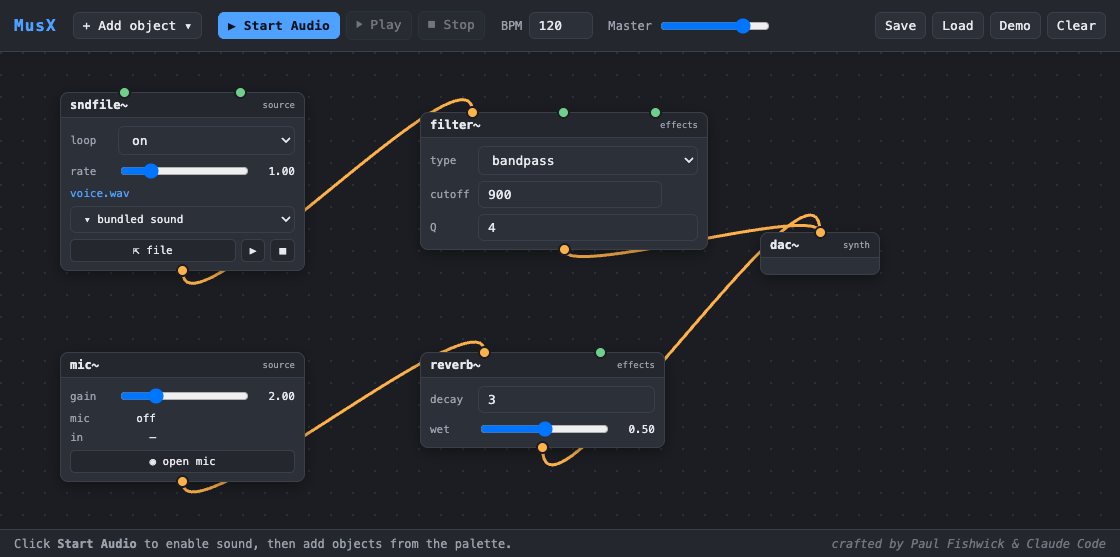
\includegraphics[width=0.9\textwidth]{source-nodes.png}
\caption{The two sound-input objects. \texttt{sndfile\~{}} (with a bundled sound loaded)
feeds a bandpass \texttt{filter\~{}}; \texttt{mic\~{}} feeds a \texttt{reverb\~{}}; both
reach the output.}
\label{fig:source-nodes}
\end{figure}

\subsection{Granular Transformation}
The granular objects granulate a buffer using overlapping short grains, which decouples
time from pitch. \texttt{grain\~{}} is the full cloud (grain size, overlap, scan speed,
transposition, reverse); \texttt{tstretch\~{}} changes speed while preserving pitch; and
\texttt{pshift\~{}} transposes while preserving speed. Figure~\ref{fig:granular-cloud}
shows two granular voices feeding a shared reverb. Because a granular object reads its own
buffer (rather than a live stream), it loads a file exactly as \texttt{sndfile\~{}} does.

\begin{figure}[h]
\centering
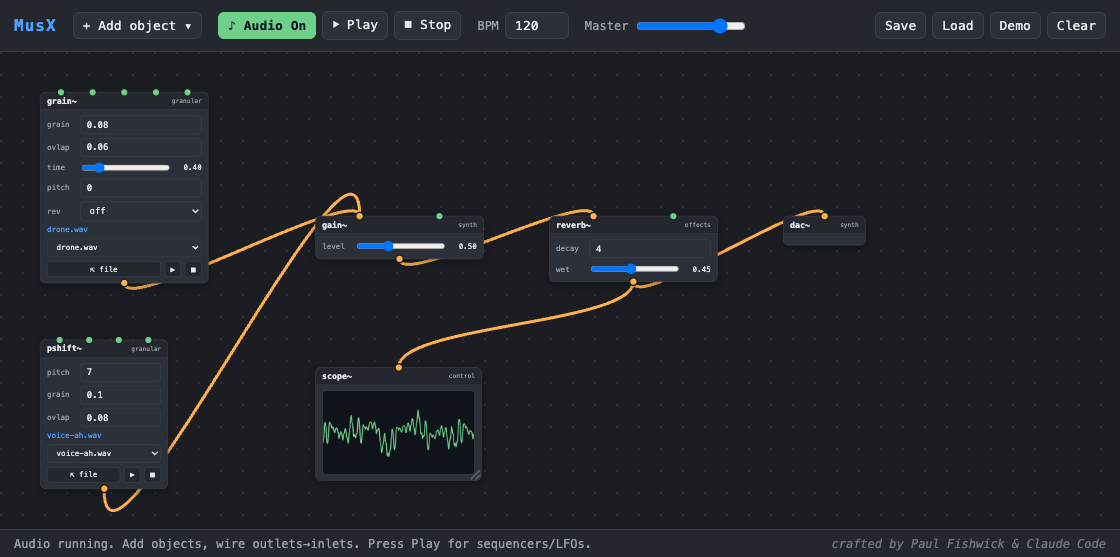
\includegraphics[width=0.9\textwidth]{granular-cloud.png}
\caption{The ``Granular Cloud'' patch (\texttt{patches/granular/}): \texttt{grain\~{}}
scans a drone slowly while \texttt{pshift\~{}} transposes a vowel up a fifth; both are
mixed into a reverb, with a \texttt{scope\~{}} on the output.}
\label{fig:granular-cloud}
\end{figure}

\subsection{Waveset Distortion}
\label{sec:waveset}
A \emph{waveset} is the fragment of a signal between alternate zero-crossings---from one
upward zero-crossing to the next. For a pure tone this is one cycle; for complex sound it
is a ``pseudo-cycle''. CDP's \textsc{distort} family rebuilds a sound from transformed
wavesets, and \texttt{wsdistort\~{}} reimplements it in real time on the live stream. A
single \emph{mode} menu selects the transformation:
\begin{itemize}
\item \textbf{repeat} --- emit each waveset several times (\emph{count}); time-extends the
sound and adds a sub-octave buzz.
\item \textbf{omit} --- keep some wavesets and drop others (\emph{keep}/\emph{skip}) for
rhythmic gating and thinning.
\item \textbf{reverse} --- reverse each waveset in place, adding grit at constant length.
\item \textbf{average} --- replace a group of wavesets with their averaged shape, smearing
timbre and pitch.
\item \textbf{telescope} --- squeeze a \emph{group} of wavesets into one, contracting time
and raising pitch.
\item \textbf{reform} --- substitute a simple waveform (\emph{shape}) scaled to each
waveset's length and peak, swapping timbre while keeping the rhythm.
\end{itemize}
The \emph{group} parameter sets how many consecutive wavesets an operation treats as a unit
(CDP's \texttt{cyclecnt}), and \emph{level} is an output gain. Because \texttt{repeat},
\texttt{omit}, and \texttt{telescope} change the number of samples, the object buffers its
output internally; the buffer is bounded (about one second) so latency cannot grow without
limit---the one concession that a live implementation makes to CDP's offline processing.
Figure~\ref{fig:waveset-crunch} shows the object crunching a sustained drone. The
distortion is 100\,\% wet, matching CDP; patch a parallel path if a dry blend is wanted.

\begin{figure}[h]
\centering
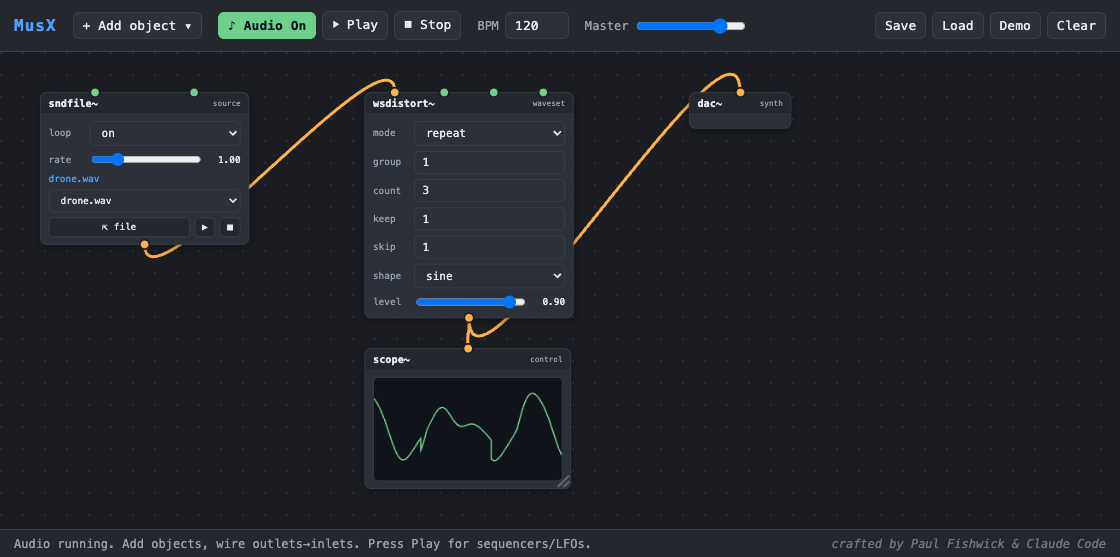
\includegraphics[width=0.9\textwidth]{waveset-crunch.png}
\caption{The ``Waveset Crunch'' patch (\texttt{patches/cdp/}): \texttt{sndfile\~{}}
auto-loads a drone into \texttt{wsdistort\~{}}, whose transformed output reaches the
speakers and a \texttt{scope\~{}}. The \emph{mode} menu selects the waveset operation.}
\label{fig:waveset-crunch}
\end{figure}

\subsection{Spectral Transformation (Phase Vocoder)}
\label{sec:spectral}
The spectral objects work in the frequency domain. The browser's analysis node can read
a spectrum but cannot resynthesize one, so MusX includes a real \emph{phase vocoder} built
as a custom audio worklet: a sliding Short-Time Fourier Transform (2048-point FFT, 75\,\%
overlap, Hann window) analyses the signal into magnitude and phase per frequency bin, an
operation modifies those bins, and an inverse transform with overlap-add reconstructs a
continuous stream. Because the transform window is finite, the objects add about 35\,ms of
latency. All five are audio-in $\to$ audio-out and leave the sound's \emph{duration}
unchanged.
\begin{itemize}
\item \texttt{spec.freeze\~{}} --- captures one spectral frame and holds it indefinitely,
advancing each bin's phase at its analysed frequency so the freeze sustains smoothly rather
than buzzing. Toggle \emph{freeze}; send a \texttt{trig} to re-capture the current sound.
\item \texttt{spec.blur\~{}} --- averages each bin's magnitude over the last N frames
(\emph{frames}), smearing transients and movement into a sustained wash.
\item \texttt{spec.filter\~{}} --- a spectral gate that keeps only bins louder than a
fraction of the frame's peak (\emph{thresh}); \emph{invert} keeps the quiet bins instead,
for denoising or for isolating a noise bed.
\item \texttt{spec.pitch\~{}} --- transposes by estimating each bin's true frequency from
its phase advance and moving it to a new bin, so pitch changes (\emph{semis}) while speed
and duration stay fixed. This is genuine pitch-shifting, distinct from varispeed.
\item \texttt{spec.stretch\~{}} --- stretches the spacing of the partials along the
frequency axis (\emph{stretch}): above 1 the overtones spread apart, turning a harmonic
tone inharmonic and bell-like; below 1 they compress. This is a \emph{spectral} stretch,
not a time-stretch (for time-stretch use the granular \texttt{tstretch\~{}}), and so it too
leaves duration unchanged.
\item \texttt{spec.morph\~{}} --- takes \emph{two} audio inputs (\emph{a} and \emph{b}) and
interpolates their spectra --- both magnitudes and per-bin frequencies --- by \emph{morph}
(0 = a, 1 = b). Unlike a gain crossfade, which simply plays two sounds at once in the
middle, this builds a genuine hybrid spectrum, so a voice can turn gradually into a bell.
\end{itemize}
Figure~\ref{fig:spectral-stretch} shows the partial-stretch object turning a drone into a
bell. All of these parameters are modulatable, so an LFO or envelope can sweep the blur
window, freeze threshold, transposition, or stretch amount over time.

\begin{figure}[h]
\centering
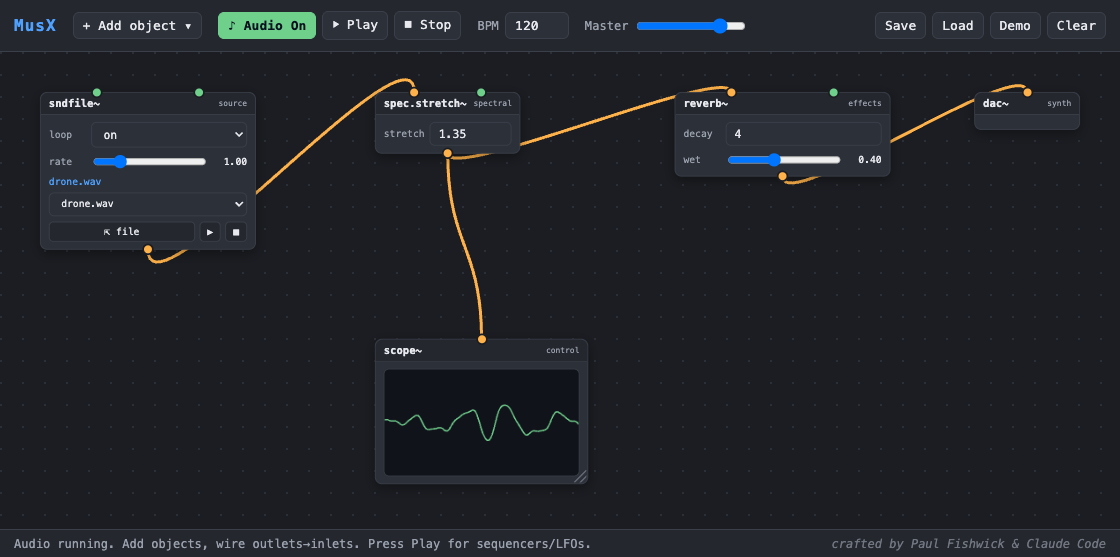
\includegraphics[width=0.9\textwidth]{spectral-stretch.png}
\caption{The ``Spectral Stretch'' patch (\texttt{patches/cdp/}): \texttt{sndfile\~{}}
auto-loads a drone into \texttt{spec.stretch\~{}}, whose inharmonic output passes through a
\texttt{reverb\~{}} to the speakers and a \texttt{scope\~{}}.}
\label{fig:spectral-stretch}
\end{figure}

\subsection{Extend, Modify, and Envelope}
\label{sec:extend}
A final family reshapes sound in the time domain and works with amplitude envelopes.

\emph{Envelope objects.} \texttt{envfollow\~{}} tracks the amplitude envelope of its input
and offers it two ways: as an audio-rate signal on \texttt{env} (to drive another object's
level) and as a 0--1 control stream on \texttt{val} (to plot or to modulate a parameter).
\texttt{envimpose\~{}} is a voltage-controlled amplifier: it multiplies a carrier by an
incoming envelope. Patching \texttt{envfollow\~{}} on a drum loop into
\texttt{envimpose\~{}} on a sustained pad makes the pad speak the rhythm of the drums, as in
Figure~\ref{fig:env-impose}.

\emph{Breakpoint automation.} \texttt{breakpoint\~{}} provides the real-time equivalent of a
CDP breakpoint file: a small canvas holding a line-segment curve that is edited by hand ---
click to add a point, drag to move it, right-click to delete --- with the two endpoints
pinned in time. When the transport runs, a playhead sweeps the curve over \emph{dur} seconds
(looping or one-shot) and emits the interpolated value, scaled to \emph{lo}--\emph{hi}, on
its \texttt{val} outlet. Wired into any modulatable parameter it becomes a drawable
automation lane; the curve is saved with the patch.

\emph{Extend / glitch objects.} \texttt{iterate\~{}} continuously records its input and, when
it receives a \texttt{trig}, grabs the last \emph{seg} milliseconds and repeats it \emph{count}
times, each repeat quieter (\emph{decay}) and transposed by a \emph{pitch} step --- a
triggered stutter or echo burst. \texttt{scramble\~{}} chops the input into \emph{seg}-length
segments, keeps the most recent few, and replays them in shuffled or drunk-walk order; it
emits one segment for every segment it records, so it stays locked to real time rather than
drifting.

\begin{figure}[h]
\centering
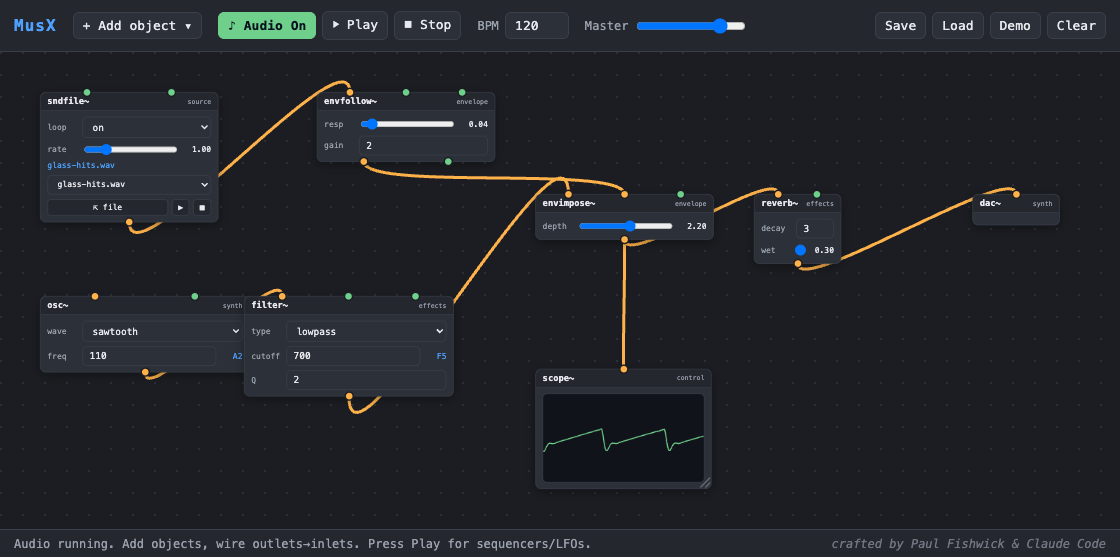
\includegraphics[width=0.9\textwidth]{env-impose.png}
\caption{The ``Envelope Impose'' patch (\texttt{patches/cdp/}): a percussive
\texttt{sndfile\~{}} drives \texttt{envfollow\~{}}, whose envelope opens the
\texttt{envimpose\~{}} VCA on a sustained saw pad, so the pad pulses in the rhythm of the
source.}
\label{fig:env-impose}
\end{figure}

\subsection{Modulatable Parameters}
\label{sec:mod}
Any parameter may be declared \emph{modulatable}, in which case it exposes an optional
control inlet named after the parameter. A cable from a \texttt{funcgen} LFO, a
\texttt{slider}, or an \texttt{xy pad} then drives that parameter continuously, while its
own widget still works when nothing is patched. For example, wiring a slow \texttt{funcgen}
into the \texttt{rate} inlet of \texttt{sndfile\~{}} automates the tape-style varispeed
wobble that is expressive to perform by hand. Modulation drives the audio directly and does
not move (or overwrite) the widget's stored value, so the effect is heard rather than seen.
The granular objects expose their grain, overlap, rate, and pitch parameters this way ---
patching an LFO into \texttt{pshift\~{}}'s pitch inlet, for instance, produces vibrato ---
and \texttt{wsdistort\~{}} likewise exposes its \emph{group}, \emph{count}, and
\emph{level} parameters, so a slow ramp into \emph{count} sweeps the waveset repetition.

\subsection{Sample Library and Grouped Patches}
Sample sounds ship under \texttt{sounds/}, organised into sub-directories
(\texttt{tonal/}, \texttt{vocal/}, \texttt{texture/}) whose names become the group
headings in the soundfile dropdown. Example patches ship under \texttt{patches/}, likewise
grouped into sub-directories (\texttt{cdp/}, \texttt{granular/}, \texttt{live/}). A patch
may reference a bundled sound by its path so that the sound auto-loads when audio starts;
saved patches store this path (not the audio itself), so bundled sounds reload
automatically while a user's own imported files are re-selected on load.

\section{The \texttt{funcgen} Expression Language}
\label{sec:funcgen}

The \texttt{funcgen} object generates a function specified algebraically, in the spirit of
Max's \texttt{expr\~{}}. The expression is written in terms of a phase variable \texttt{t}.
It is evaluated two ways simultaneously: the \texttt{sig} outlet plays one cycle of the
expression over \texttt{t}$\,\in[0,1)$ as an audible wavetable oscillator, and the
\texttt{val} outlet samples the expression over time as a control stream suitable for
feeding a \texttt{plot} (Figure~\ref{fig:funcgen-plot}). The parser is sandboxed --- it
never calls JavaScript \texttt{eval} on user input --- and supports \texttt{+ - * / \^{}},
parentheses, the constants \texttt{pi}, \texttt{e}, \texttt{tau}, and the functions
\texttt{sin cos tan asin acos atan exp log ln sqrt abs floor ceil round sign min max mod}
plus oscillator shapes \texttt{saw square tri pulse}.

\begin{figure}[h]
\centering
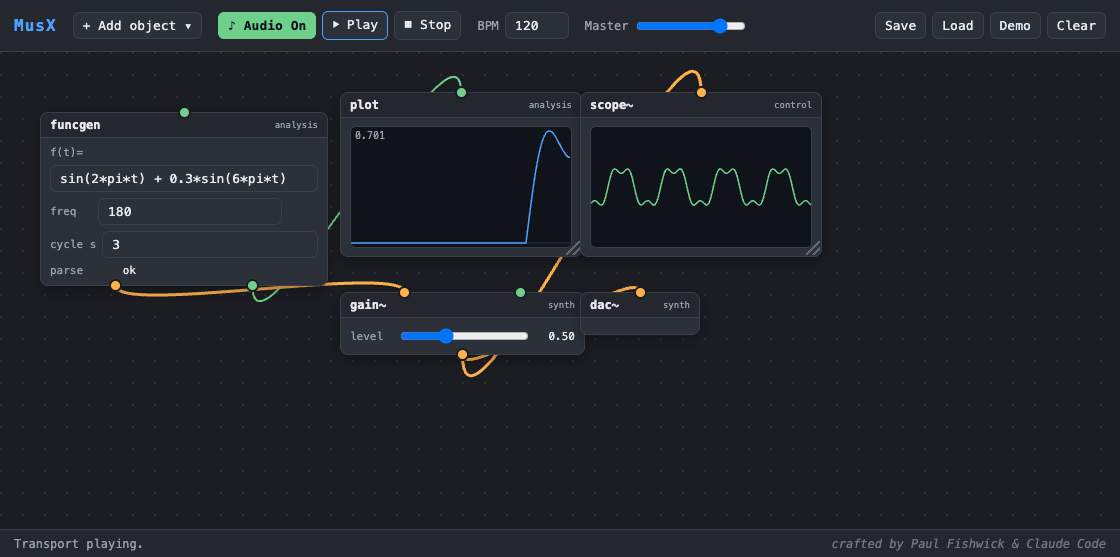
\includegraphics[width=0.85\textwidth]{funcgen-plot.png}
\caption{A \texttt{funcgen} evaluating \texttt{sin(2*pi*t) + 0.3*sin(6*pi*t)}. The
\texttt{plot} (blue) shows the function sampled over time; the \texttt{scope\~{}} (green)
shows the same function rendered as an audible wavetable --- note the matching harmonic
ripple.}
\label{fig:funcgen-plot}
\end{figure}

\section{Code Objects}
\label{sec:code}

The \texttt{code} object runs user-written code at control rate: it reads its inlets
\texttt{a} and \texttt{b}, runs the code whenever an input arrives, and emits the result.
Two languages are supported. \textbf{JavaScript} runs natively (a bare expression such as
\texttt{a*b+1} or a function body with \texttt{return}). \textbf{Python} runs through the
Pyodide WebAssembly runtime~\cite{pyodide}, which is downloaded from its CDN the first time
a Python code object executes; JavaScript code objects never trigger that download.
Figure~\ref{fig:bang-code} shows a patch in which a \texttt{message} sends a MIDI number to
a \texttt{code} object that converts it to hertz, while a \texttt{bang} button triggers the
envelope.

\begin{figure}[h]
\centering
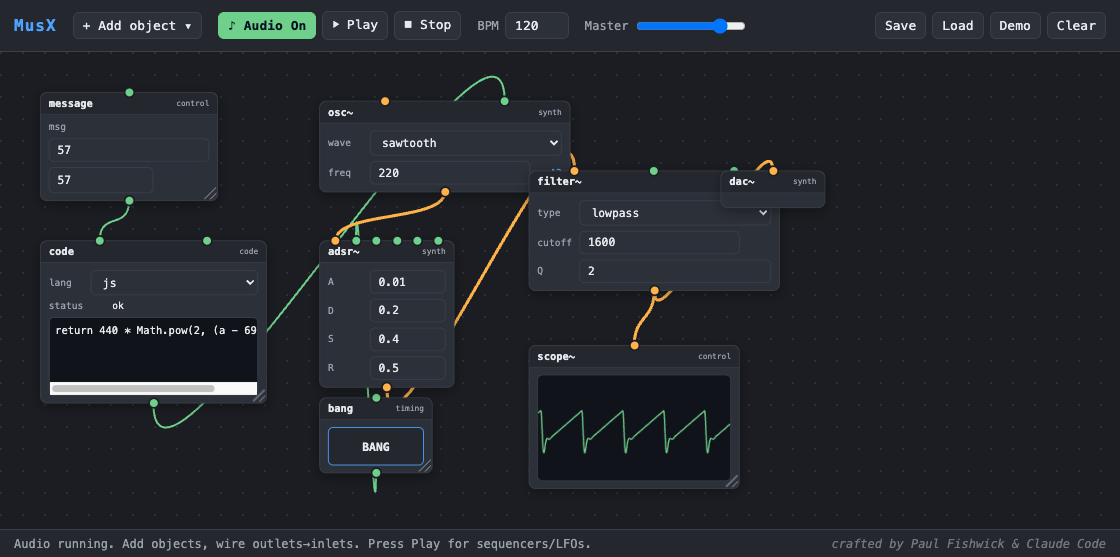
\includegraphics[width=0.95\textwidth]{bang-code.png}
\caption{The ``Bang + Code'' patch. A \texttt{message} (MIDI 57) feeds a \texttt{code}
object computing \texttt{440 * Math.pow(2,(a-69)/12)} $\rightarrow$ the oscillator's
frequency; the \texttt{bang} button triggers the \texttt{adsr\~{}}.}
\label{fig:bang-code}
\end{figure}

\paragraph{Security note.} Because a code object executes the code it contains, loading a
patch file authored by someone else will run that code --- exactly as opening a Max patch
containing a \texttt{js} object would. This is safe for your own patches; treat untrusted
patch files with the same caution as any downloaded program.

\section{Subpatches and Abstractions}
\label{sec:subpatch}

A \texttt{patcher} object is a box whose \emph{inside} is another patch, so a group of objects
can be reused as a single block --- the MusX equivalent of a Max sub-patch or Pd abstraction.
Double-clicking a \texttt{patcher} \textbf{descends} into its inner graph; a breadcrumb trail at
the top-left of the canvas (\texttt{root patch} $\triangleright$ \texttt{patcher}) shows the current depth, and
clicking a breadcrumb segment \textbf{climbs} back out. Nesting is arbitrary --- patchers may
contain patchers.

The box's ports are defined by \emph{boundary objects} placed inside it: each \texttt{inlet\~{}}
or \texttt{inlet} adds one input port (audio or control) and each \texttt{outlet\~{}} or
\texttt{outlet} adds one output, ordered left-to-right by position. The engine runs a patcher as
a nested runtime: audio and control cross the boundary transparently, so a subpatch behaves
exactly like a hand-built chain (Figure~\ref{fig:subpatch}).

\paragraph{Encapsulating a selection.} Rather than building a box from scratch, several existing
objects can be collapsed into one. Shift-click objects (or shift-drag a rubber-band box) to
multi-select, then press \texttt{Cmd/Ctrl+E} or the \textbf{Encapsulate} toolbar button. MusX
moves the selected objects into a new \texttt{patcher}, automatically creating a boundary object
for every cable that crossed the selection and rewiring those cables to the new box's ports.
Any object can be \emph{renamed} by double-clicking its title and typing (Enter to commit, Escape
to cancel) --- most useful for giving a \texttt{patcher} a meaningful name such as
\emph{``cathedral voice''} instead of the generic ``patcher''.

\paragraph{File-referenced abstractions.} A \texttt{patcher} can instead \emph{reference} a saved
\texttt{.json} patch file under the served tree, so one definition can be instanced in many
places. The three actions live in the toolbar's \textbf{Abstractions} dropdown: \emph{Insert
abstraction} creates such a box from a path; \emph{Save as abstraction} downloads the current
subpatch as a reusable file; and \emph{Reload abstractions} re-fetches
every referenced file so an edit to the definition propagates to all instances at once. A
referenced box is read-only when opened (a banner marks it so), with a \textbf{Detach} action to
fork it into a private, editable inline copy.

\begin{figure}[h]
\centering
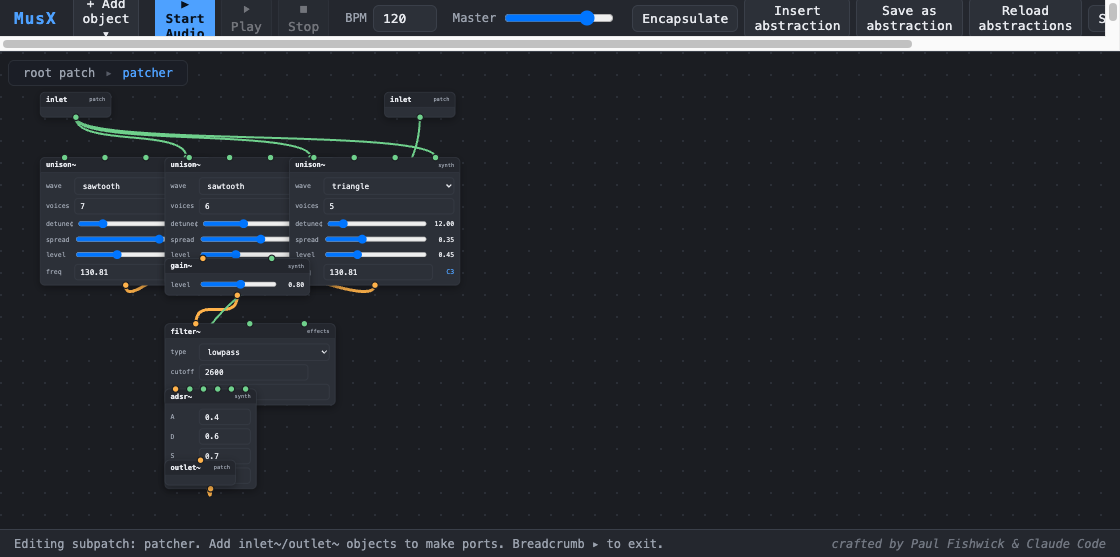
\includegraphics[width=0.95\textwidth]{subpatch.png}
\caption{A \texttt{patcher} opened for editing. The breadcrumb (top-left) shows
\texttt{root patch} $\triangleright$ \texttt{patcher}; inside, \texttt{inlet}/\texttt{outlet\~{}} boundary
objects define the box's ports while the inner objects do the work.}
\label{fig:subpatch}
\end{figure}

\section{Fat Synth Voices: Unison, Panning, and Chords}
\label{sec:richsound}

Rich, wide, ``cinematic'' synth textures come less from adding more oscillators than from a
specific architecture: \emph{unison voice stacking}, \emph{detuning}, and \emph{stereo
spreading} (and, for sampled sources, a randomised start time). MusX packages this as a small
family of objects, inspired by the layered-oscillator design of instruments such as
Hexeract~\cite{hexeract}.

\paragraph{\texttt{unison\~{}}.} A single oscillator \emph{module} that internally runs up to
eight voices of the chosen waveform. Each voice is detuned by a symmetric offset in \emph{cents}
(so the perceived width is the same at every pitch) and placed at its own position across the
stereo field by an equal-power panner; the voices are summed with a $1/\sqrt{N}$ scaling to keep
loudness roughly constant as the count changes. Its parameters are \texttt{wave}, \texttt{voices}
(1--8), \texttt{detune} (cents), \texttt{spread} (0--1), and \texttt{level}; a single \texttt{freq}
control fans out to all voices, and changing the voice count rebuilds the stack live. One
\texttt{unison\~{}} already sounds like a small ensemble; stacking a few (with different waveforms
and detune amounts) yields the classic ``supersaw'' pad.

\paragraph{\texttt{pan\~{}}.} A plain equal-power stereo panner, useful for placing any mono
source in the field or for widening a hand-built stack.

\paragraph{\texttt{spat\~{}}.} A 3D binaural panner built on the Web Audio HRTF
model (\texttt{Tone.Panner3D})~\cite{webaudio}. The listener sits at the origin facing
$-z$; three controls place the source in space: \texttt{x} left($-$)/right($+$),
\texttt{y} down($-$)/up($+$), and \texttt{z} front($-$)/back($+$). Heard over headphones the
source is localized in three dimensions, not just across the stereo pair. Because each of
\texttt{x}, \texttt{y}, \texttt{z} is modulatable, wiring an \texttt{xy pad} or a slow
\texttt{funcgen} into them sweeps a sound around the head in real time. (For a single moving
source this HRTF panner is the natural fit; a full rotatable \emph{soundfield}, e.g.\ for VR
head-tracking, would call for an Ambisonics stage, a possible future addition.)

\paragraph{\texttt{chord}.} Turns one \texttt{root} frequency into a chord. A \texttt{quality}
control selects \emph{major, minor, augmented, diminished, sus2,} or \emph{sus4}, and a
\texttt{notes} control selects how many notes sound: just the \emph{root}, a \emph{power} chord
(root + fifth), a \emph{triad} (1--3--5), or a \emph{7th} (1--3--5--7). The chord tones are
distributed across four frequency outlets, wrapping when there are fewer tones than outlets so
that every connected voice always receives a sensible pitch --- selecting \emph{root} therefore
simply doubles the root, making the chord entirely optional. The chord recomputes live as the
root arrives or the quality/size change, so it can be reshaped while a note is held.

\paragraph{Start-Mod for samples.} Stacking several copies of the \emph{same} sample in unison
causes hollow, metallic phase cancellation. The \texttt{sndfile\~{}} object's \texttt{startmod}
parameter applies a small random start-time offset (0--200\,ms) on each trigger, so stacked
sample voices blend into a lush ensemble instead of cancelling.

\paragraph{Hold to sustain.} The on-screen \texttt{keyboard} plays gated notes: pressing a key
opens and \emph{sustains} the envelope, and releasing it triggers the release --- so a held key
sounds for as long as it is held. The \texttt{adsr\~{}} envelope honours these note-on/note-off
messages, while the \texttt{note} object and step sequencer keep their original fixed-duration
triggering.

\paragraph{Piano-roll sequencing (\texttt{pianoroll}).} Where \texttt{step seq} is an eight-row
scale grid, the \texttt{pianoroll} object is a full piano-roll track sequencer: notes of any pitch
and length are drawn on a time~$\times$~pitch canvas and played back in sync with the transport,
driving one voice through the same \texttt{freq}~+~\texttt{trig} outlets as the keyboard. Click-drag
empty space to draw a note (the drag sets its length), drag a note to move it, drag its right edge
to resize, Shift-drag vertically to set velocity (which feeds the \texttt{adsr\~{}} \texttt{veldb}
curve), and right-click to delete; the box is resizable for a larger editing surface. Playback uses
a looping \texttt{Tone.Part}. The design follows the piano-roll editor XPianoRoll~\cite{xpianoroll}
(which is only the editor GUI --- \emph{``a sequencer is not part of XPianoRoll''}); the MusX object
bundles editor and playback. The built-in \textbf{Piano Roll (Silo melody)} demo pre-loads the
first eight-bar phrase of the Silo violin line (decoded from its MIDI file with the exact timing,
transposed down an octave) and drives the Cathedral Pad voice, which is packaged as a
file-referenced abstraction (\texttt{patches/abstractions/cathedral-voice.json}) named
\emph{``cathedral voice''} --- so the top level is just three boxes: roll, voice, and \texttt{dac\~{}}.

\paragraph{Sampled voices (\texttt{sampler\~{}}).} The fat, ``cinematic'' side of instruments
like Hexeract is largely \emph{sample}-driven: real recordings (choirs, strings, brass) played
back per key. The \texttt{sampler\~{}} object provides this --- it plays a loaded sample at a
playback rate set by the incoming \texttt{freq} relative to a \texttt{root} pitch
(varispeed), with a built-in attack/release gate so a held key sustains (looping the sample) and
releases cleanly, plus the same Start-Mod jitter for stacking. To sustain smoothly, the loop's
seam is equal-power crossfaded and its start (\texttt{loop\ensuremath{\rightarrow}}, in
milliseconds) is moved past the onset attack, so the loop sits in the steady-state part of the
sample rather than re-triggering the attack each cycle. Crucially, because it is driven by
\texttt{freq} exactly like an oscillator, it drops into the same \texttt{keyboard}~+~\texttt{chord}
rig: replacing the synth voices with \texttt{sampler\~{}} voices turns the chord patch into a
\emph{sampled} chord with no other change (see the demos below).

\section{Built-in Demo Patches}

Nine demos ship with MusX. Two reproduce examples from the Max/MSP product
page~\cite{maxmsp}. \textbf{Custom Synth} (Figure~\ref{fig:custom-synth}) recreates the
first ``Sound without limits'' patch: stacked saw and square oscillators through a resonant
filter, distortion, and delay, driven by the step sequencer. \textbf{Layered Pad}
(Figure~\ref{fig:layered-pad}) recreates the third patch, which in Max uses multichannel
(MC) objects to stack fifty detuned oscillators; MusX emulates this with a stack of detuned
oscillators feeding an LFO-swept filter and reverb. \textbf{Richsound Chord}
(Figure~\ref{fig:richsound}) shows the fat-voice objects at work: a \texttt{keyboard} drives a
\texttt{chord} object whose tones set three \texttt{unison\~{}}-based voices (each a referenced
\emph{richsound} abstraction, Section~\ref{sec:subpatch}), so a single held key sustains a wide,
transposable chord (Section~\ref{sec:richsound}). Two further demos show the sampled path: \textbf{Sampler (playable)} plays a bundled ``ah'' vowel
chromatically from the keyboard, and \textbf{Sampled Chord} is the identical keyboard~+~\texttt{chord}
rig with the three voices replaced by \texttt{sampler\~{}} objects, giving a choir-like sampled
chord. \textbf{3D Orbit} sends a bright sawtooth through \texttt{spat\~{}} while two \texttt{funcgen}
LFOs circle it around the listener (put on headphones), and \textbf{Cathedral Pad} is a playable
version of the full ``fat \& massive'' recipe: a keyboard feeds a \texttt{chord} that pitches
two detuned \texttt{unison\~{}} voices to the played root and fifth, a \texttt{math} node drops a
sine an octave below for sub weight, and an \texttt{adsr\~{}} (sustain~$=1$) holds the sound for
as long as the key is down. The signal is tamed by a lowpass and gently saturated, then sent to a
long, pre-delayed \texttt{reverb\~{}} whose send is high-passed for a clean tail.
\textbf{Cathedral (MIDI, polyphonic)} plays a real \texttt{.mid} file through a bank of eight
Cathedral voices: the \texttt{midifile} object parses the file, and its built-in voice allocator
hands each note to a free voice (one \texttt{freq}/\texttt{trig} outlet pair per voice, exactly
like the keyboard), so the piece sounds as actual chords summed into one shared reverb.
\textbf{Cathedral (MIDI, monophonic)} plays the same file through the single mono pad instead:
the \texttt{midifile} object's \texttt{mode} is set to \emph{mono}, so it follows the highest held
note and keeps the gate open through overlaps (legato), turning the dense piece into one
continuous, evolving line — cleaner than the polyphonic version, which can wash out where the
music is busiest. Both demos also carry a \emph{credit}: patches may include an optional
\texttt{credits} field (\texttt{text} + \texttt{url}) that the viewer shows in a small box in the
top-right corner. The \texttt{midifile} object's \texttt{track} (isolate one part),
\texttt{start} (skip seconds), \texttt{mode} (poly/mono), and \texttt{retrig} controls make its
playback configurable live. The remaining demos are \textbf{XY Synth}
(Figure~\ref{fig:interface}), \textbf{FuncGen $\rightarrow$ Plot} (Figure~\ref{fig:funcgen-plot}),
\textbf{Keyboard Synth}, and \textbf{Bang + Code} (Figure~\ref{fig:bang-code}).

\begin{figure}[h]
\centering
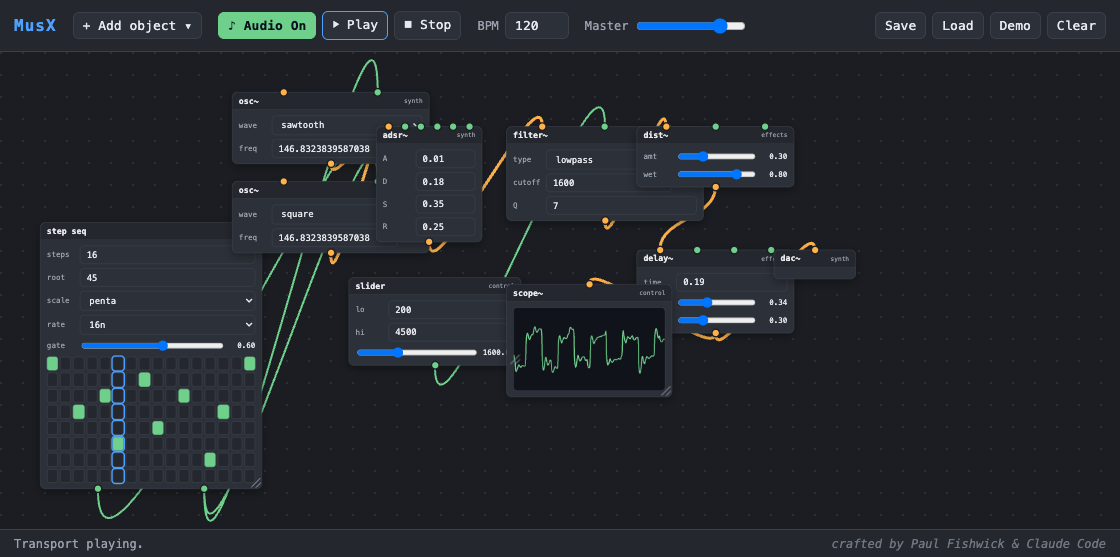
\includegraphics[width=0.95\textwidth]{custom-synth.png}
\caption{The ``Custom Synth'' demo (Max ``Sound without limits'', patch~1): a step
sequencer drives saw + square oscillators through an envelope, resonant lowpass filter,
distortion, and delay, with a scope on the output.}
\label{fig:custom-synth}
\end{figure}

\begin{figure}[h]
\centering
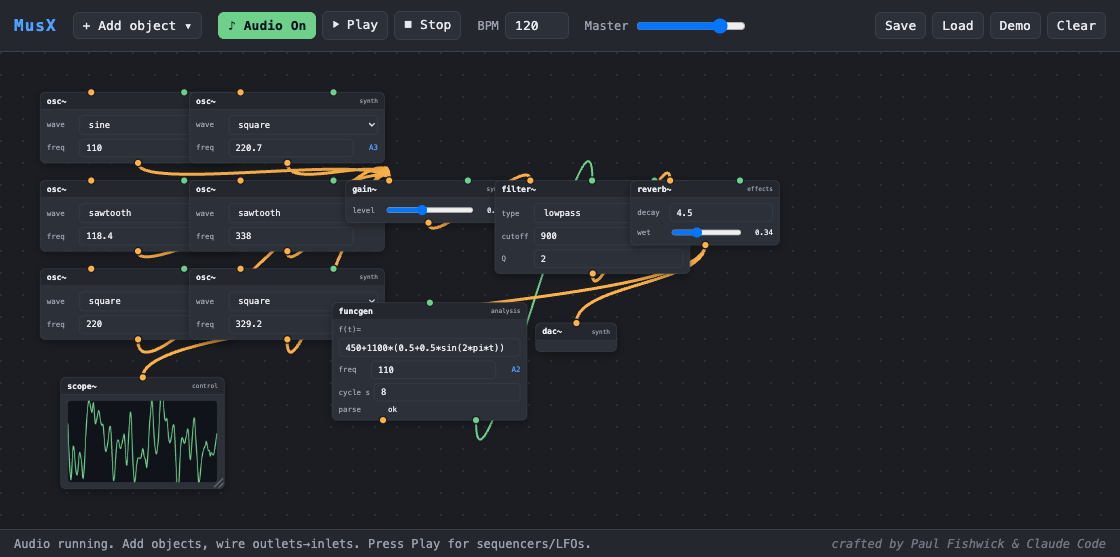
\includegraphics[width=0.95\textwidth]{layered-pad.png}
\caption{The ``Layered Pad'' demo (Max ``Sound without limits'', patch~3): six detuned
oscillators are mixed and passed through a filter whose cutoff is swept by a slow
\texttt{funcgen} LFO, then reverberated. This emulates the MC (multichannel) oscillator
bank of the original.}
\label{fig:layered-pad}
\end{figure}

\begin{figure}[h]
\centering
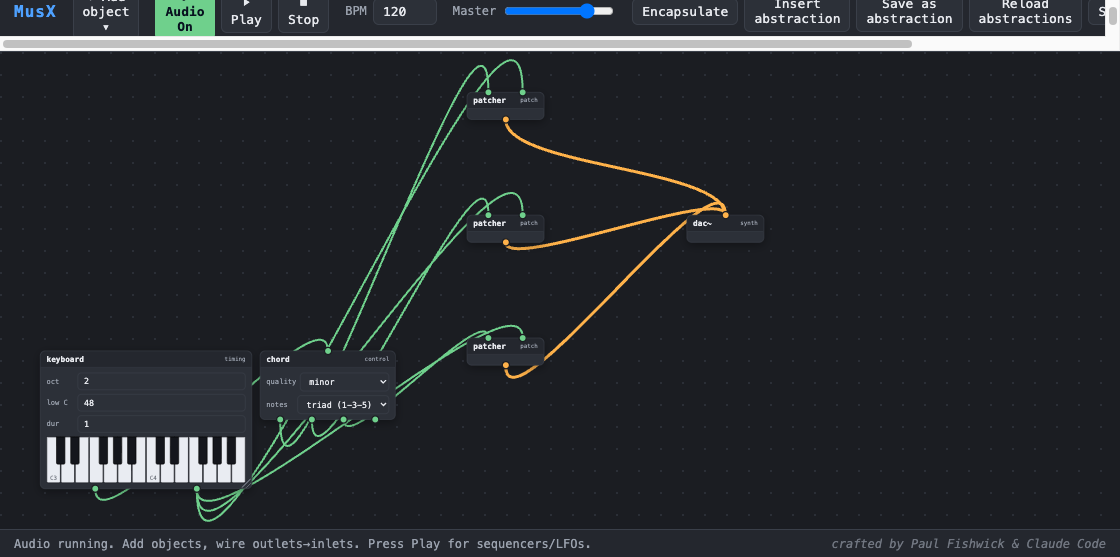
\includegraphics[width=0.95\textwidth]{richsound.png}
\caption{The ``Richsound Chord'' demo: a \texttt{keyboard} feeds a \texttt{chord} object, whose
four frequency outlets drive three \texttt{unison\~{}}-based voices (referenced \emph{richsound}
abstractions). The one keyboard gate holds all three envelopes, so a held key sustains a wide,
transposable chord; the chord object's quality and size can be changed live.}
\label{fig:richsound}
\end{figure}

\section{Architecture}

MusX separates two layers. The \emph{graph layer} (\texttt{js/graph/}) holds a serialisable
model of objects and connections and renders the boxes, ports, and cables; it knows nothing
about audio. The \emph{audio layer} (\texttt{js/audio/engine.js} plus the per-object
definitions in \texttt{js/nodes/}) builds the live Tone.js~\cite{tonejs} graph from the
model. Audio cables become real Tone connections; control cables are delivered dynamically
--- when an object emits, the engine looks up the current control connections and calls the
targets --- so editing cables while running takes effect immediately. A single master gain
node sits between every \texttt{dac\~{}} and the Web Audio destination~\cite{webaudio}; the
transport's Stop ramps it to zero, which is how Stop reliably silences free-running drones.

\section{Developer Reference: Adding a New Object}
\label{sec:dev}

An object type is one entry in the node registry. A definition declares its title,
category, inlets, outlets, parameter widgets, an optional \texttt{render} for custom UI,
and a \texttt{create} that builds its Tone.js object(s) and returns a small runtime
(\texttt{audioIn}, \texttt{audioOut}, \texttt{receive}, \texttt{setParam}, \texttt{start},
\texttt{dispose}). To make an object resizable, set \texttt{resizable: true} and, in
\texttt{render}, assign \texttt{view.\_vizEl} (the element to measure) and
\texttt{view.\_onResize(w, h)} (how to apply a new size). No change to the graph engine is
required.

\section{Testing}

MusX ships with a headless test harness (\texttt{tests/auto/test.mjs}) that loads each demo
and verifies both structure and sound. Because a browser cannot ``hear'' audio, the harness
taps a meter off the master and reads the live level in decibels, confirming that a patch
produces real signal rather than silence, that Stop drives the output to zero, and that the
keyboard and bang trigger audible notes. The manual's figures are produced separately by a
Selenium script (\texttt{docs/make\_figures.py}) that drives the same interface in headless
Chrome.

\begin{thebibliography}{9}
\bibitem{puckette} M.~Puckette. ``Pure Data: another integrated computer music
  environment.'' \emph{Proceedings of the International Computer Music Conference}, 1996.
  Software: \url{https://puredata.info}.
\bibitem{maxmsp} Cycling~'74. \emph{Max} (Max/MSP). \url{https://cycling74.com/products/max}.
\bibitem{webaudio} W3C. \emph{Web Audio API}. \url{https://www.w3.org/TR/webaudio/}.
\bibitem{tonejs} Y.~Mann. \emph{Tone.js: A Web Audio framework for interactive music in the
  browser}. \url{https://tonejs.github.io}.
\bibitem{pyodide} The Pyodide development team. \emph{Pyodide: Python with the scientific
  stack, compiled to WebAssembly}. \url{https://pyodide.org}.
\bibitem{cdp} The Composers Desktop Project. \emph{CDP: a suite of sound-transformation
  processes for \emph{musique concr\`ete}}. \url{https://www.composersdesktop.com};
  source: \url{https://github.com/ComposersDesktop/CDP8}.
\bibitem{soundthread} J.-P.~Higgins. \emph{SoundThread: a node-based graphical interface
  for the Composers Desktop Project}. \url{https://github.com/j-p-higgins/SoundThread}.
\bibitem{hexeract} HeavyMetal. \emph{Hexeract: a layered-oscillator software synthesizer}.
  Cited as the design inspiration for the fat unison/detune/spread voice architecture.
\bibitem{sugiyama} K.~Sugiyama, S.~Tagawa, and M.~Toda. ``Methods for visual understanding of
  hierarchical system structures.'' \emph{IEEE Transactions on Systems, Man, and Cybernetics},
  11(2):109--125, 1981. \url{https://doi.org/10.1109/TSMC.1981.4308636}.
\bibitem{gansner} E.~R.~Gansner, E.~Koutsofios, S.~C.~North, and K.-P.~Vo. ``A technique for
  drawing directed graphs.'' \emph{IEEE Transactions on Software Engineering}, 19(3):214--230,
  1993. \url{https://doi.org/10.1109/32.221135}.
\bibitem{xpianoroll} X.~Roemer. \emph{XPianoRoll: a piano-roll MIDI editor for Max/MSP}. MIT
  License. \url{https://github.com/XRoemer/XPianoRoll}. Cited as the design inspiration for the
  \texttt{pianoroll} object's editing surface.
\end{thebibliography}

\end{document}
